\section{Test data generation for direct mapped cache}

\begin{figure}[h]
\centering
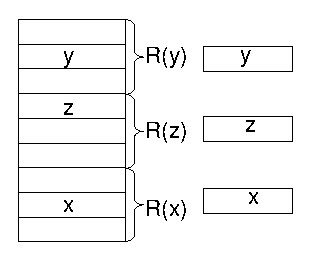
\includegraphics[width=2.5in]{prm}
\caption{Direct mapped cache} \label{prm_pic}
\end{figure}

Whole memory is divided into non-intersecting areas
(\emph{regions}). Direct mapped cache consists of 1 cell for each
region. Each cache cell may store data only from its region. Access
to memory starts from access to cache. \emph{Cache hit} means
successful match cached address with required address in its region.
\emph{Cache miss} means unsuccessful match cached address with
required address in its region. In this case data from cache
replaced by data from memory by required address.

Proposed algorithm generates constraints on the following variables:
\begin{enumerate}
\item $\alpha_1, \alpha_2, \alpha_3,...$ are addresses of the initial
cache state (their count is regions' count);
\item hits-addresses (addresses of instructions from test templates
with cache hit test situation);
\item misses-addresses (addresses of instructions from test templates
with cache miss test situation);
\item evicted addresses (evicted addresses of instructions from test templates
with cache miss test situation);
\item $L_0, L_1, ...$ -- cache states
\end{enumerate}

Define function $R(y)$ which for address $y$ returns a set of all
cells from the same region as region of $y$. $R$ satisfies the
following properties:

$\forall x~( x \in R(x) )$

$\forall x~\forall y~( x = y \rightarrow R(x) = R(y) )$

$\forall x~\forall y~( R(x) = R(y) \leftrightarrow x \in R(y) )$

$\forall x~\forall y~( R(x) = R(y) \leftrightarrow y \in R(x) )$

$\forall x~\forall y~( x \notin R(y) \rightarrow x \neq y )$

Proposed algorithm generates constraints for each instruction by the
following way ($N$ means number of regions):
\begin{enumerate}
\item "initial constraints" are generated one time for each template :
$|\{ \alpha_1, \alpha_2,..., \alpha_N\}| = N$ (other words, numbers
$\alpha_1, \alpha_2,..., \alpha_N$ are different), $|\{ R(\alpha_1),
R(\alpha_2),..., R(\alpha_N)\}| = N$ (other words, all sets
$R(\alpha_1), R(\alpha_2),..., R(\alpha_N)$ are different);
\item "hits-constraints" are generated for each instruction
with cache hit: $x \in L$, where $x$ means address from instruction,
$L$ means a current variable-state of cache memory;
\item "miss-constraints" are generated for each instruction with
cache miss ($x$ means evicting address, $y$ means evicted address,
$L$ means a current variable-state of cache): $y \in L, x \notin L,
L' = L \cup \{x\} \setminus \{y\}, R(y) = R(x)$, $L'$ became the
current variable-cache state for the next instruction.
\end{enumerate}

Constraints for direct mapped cache differ from constraints for
fully associative cache by evicted address constraints only.

Consider test data generation for the already known test template.
Lets memory divided into 3 regions depended on remainder from
division address to 3 (i.e. $R(x) = R(y) \Leftrightarrow 3 | (x-y)$
).

LOAD x, y @ Hit

STORE u, z @ Miss

LOAD z, y @ Hit

Define unique names for variables in test template (each new
variable shouldn't change its value). LOAD gives new version for its
first argument. STORE doesn't generate new version of variables.
Define new variable $z'_0$ for evicted address from the second
instruction (this variable won't be included to the solution):

LOAD $x_1, y_0$ @ Hit

STORE $u_0, z_0$ @ Miss $\rightarrow z'_0$

LOAD $z_1, y_0$ @ Hit

Define variables of initial cache state: $\{ \alpha, \beta, \gamma
\}$ (one for each region).

So the task is looking for values of $x_0, y_0, z_0, u_0, \alpha,
\beta, \gamma$ according to test template. This task has more than 1
solutions. But any solution is enough.

The first constraints describe cache hits and misses as belong to
the current state of cache:

$y_0 \in \{ \alpha, \beta, \gamma \}$,

$z_0 \notin \{ \alpha, \beta, \gamma \}$,

$z'_0 \in \{ \alpha, \beta, \gamma \}$,

$y_0 \in \{ \alpha, \beta, \gamma \} \setminus \{z'_0 \} \cup \{ z_0
\}$,

$R(z_0) = R(z'_0)$,

$\alpha, \beta, \gamma$ -- different

$R(\alpha), R(\beta), R(\gamma)$ -- different

Simplify this constraints set:

$z'_0 \in \{ \alpha, \beta, \gamma \}$,

$y_0 \in \{ \alpha, \beta, \gamma \} \setminus \{z'_0\}$,

$z_0 \notin \{ \alpha, \beta, \gamma \}$,

$ 3 | ( z_0 - z'_0 )$,

$\alpha, \beta, \gamma$ -- different

$R(\alpha), R(\beta), R(\gamma)$ -- different

Note that $x_0$ and $u_0$ don't take part in constraints. So their
values may be arbitrary.

Lets bit length of addresses is 8. So domain of all
variable-addresses is from 0 to 255. Satisfying constraints
variables can get the following values (these values are not
unique):

$\alpha = x_0 = u_0 = 0$

$\beta = y_0 = 1$

$\gamma = 2$

$z_0 = 3$

Verify test template execution with generated initial cache state
and register values:

initial cache state is $L = [(R=0) \mapsto 0, (R=1) \mapsto 1, (R=2)
\mapsto 2]$

LOAD x, 1 - Hit, because $R(1) = L[R=(1~mod~3)]$

STORE 0, 3 - Miss, because $R(3) \neq L[R=( 3~mod~3 )]$, 1 is
evicted from cache, the next state of cache is $L = [(R=0) \mapsto
0, (R=1) \mapsto 3, (R=2) \mapsto 2]$

LOAD z, 0 - Hit, because $R(0) = L[R=(0~mod~3)]$

All instructions from test template were executed according to given
test situations.
